\documentclass[man]{apa2}
\usepackage{pslatex}
\usepackage{amssymb}
\usepackage{graphicx}
\usepackage{color}
\usepackage{covington}
\usepackage[usenames,dvipsnames]{xcolor}
\usepackage{booktabs}
\usepackage{setspace}
% \usepackage{textgreek}
\usepackage{geometry}
\usepackage{pdflscape}
\usepackage{array}
\usepackage{floatrow}
\usepackage{fancyhdr}
\usepackage{cite}

\fancyhf{} % sets both header and footer to nothing
\renewcommand{\headrulewidth}{0pt}

\newcolumntype{C}[1]{>{\centering\let\newline\\\arraybackslash\hspace{0pt}}m{#1}}
\pagestyle{fancy}
\rhead{The trouble with quantifiers \ \ \thepage}
\begin{document}
~\\
~\\
~\\
%\shorttitle{The trouble with quantifiers}
%\rightheader{The trouble with quantifiers}
\begin{center}
\textbf{The trouble with quantifiers: Explaining children's deficits in scalar implicature}
\end{center}
%\author{  }
%\affiliation{  }
\newpage 
\begin{center}
\textbf{Abstract}
\vspace{5 mm}
\end{center}
\noindent
Scalar implicatures (SI) require a listener to make pragmatic inferences that extend beyond the literal meaning of an utterance (e.g., inferring from ``I ate some of the cookies'' that I ate some, but not all). Adults reliably make this pragmatic inference but children generally have more difficulty. In a supportive paradigm, three-- to five--year--olds (N = 171) can compute ad-hoc, but not scalar, implicatures (Experiment 1); implicature computation and successful comprehension of ``none'' were strongly correlated (Experiment 2). An individual differences study revealed a correlation between quantifier knowledge and implicature success (Experiment 3). Our findings suggest that SI failures may in fact be rooted in a lack of quantifier knowledge rather than general pragmatic or processing demands.

%Using language requires making pragmatic inferences that extend beyond the literal meaning of utterances. For example, ``\textit{some} of the cookies are oatmeal raisin'' carries the scalar implicature that \emph{not all} the cookies are. Adults make this pragmatic inference very reliably but children generally have more difficulty. Their performance varies tremendously across studies, however, and it is unclear how much of their difficulty stems from issues specific to quantifiers and how much comes from general pragmatic or processing demands. We designed an experimental paradigm to address this question. In Experiment 1, we measured children's ability to compute both ad-hoc (contextual) and scalar (quantifier) implicatures. While 4-year-olds were at ceiling for ad-hoc descriptions, they performed poorly using quantifiers. We also found correlated performance between the quantifiers ``some'' and ``none.''  Experiment 2 replicated this correlation in an experiment including only quantifiers. In Experiment 3 we found that inhibitory control did not predict the ability to make implicatures, but that performance across quantifier tasks was highly correlated. Our findings suggest that difficulty with scalar implicatures may in fact be rooted in a lack of quantifier knowledge.

~\\

\noindent
Keywords: scalar implicature, pragmatics, development

%\shorttitle{The trouble with quantifiers}
%\rightheader{The trouble with quantifiers}
%\acknowledgements{
%
%~\\
%
%\noindent }

%\begin{document}
%\maketitle
\newpage

\section{}

In comprehending speech, adult listeners routinely make inferences that go beyond the literal sense of an utterance. For example, an adult who hears ``I ate \emph{some} of the cookies'' would expect that the speaker did not eat \emph{all} the cookies. Similarly, an adult listener who hears ``I ate the sugar cookies,'' would most likely assume that the speaker ate \emph{only} the sugar cookies, and not the other varieties. These two statements use a weaker literal description (in these cases, scalar and contextual, respectively) to implicate that a stronger alternative is false. The first statement requires the listener to make a \emph{scalar implicature}, which relies on lexical scales such as quantifiers (``some'' vs. ``all'') or modals (``possibly'' vs. ``definitely'') \citeA{horn1972}. The second statement requires an \emph{ad-hoc implicature}, in which a stronger description is negated by a contextually weaker description; while \citeA{grice1975} distinguished ``generalized'' and ``particularized'' implicatures, this distinction has been controversial. Here we use ``ad-hoc implicature'' as a term of convenience to describe contextually-supported inferences while remaining agnostic about the theoretical distinction. Both scalar and ad-hoc implicatures are abundant in language; it would be time-consuming and costly to both a speaker and listener if all intended meaning had to be conveyed by a literal utterance. Thus, pragmatic listeners must be able to compute such implicatures readily.

How does such a critical pragmatic skill develop? While adults sometimes incur a processing cost in computing scalar implicatures along quantifier lexical scales like  $<${\sc some, all}$>$ \citeA{bott2004,grodner2010,huang2009b}, by and large they compute implicatures reliably in a wide variety of situations. In contrast, early investigations showed that children's accuracy on these same scales was variable even until fairly late in development \citeA{noveck2001}. This result was intriguing because implicatures are an important case study for children's pragmatic reasoning more generally. The finding that even elementary-aged children struggled with certain types of pragmatic judgments suggested a surprising disconnect between pragmatics and other aspects of language development.

While this early work made an important contribution by identifying an area of difficulty for children, both the use of a truth-judgment task and the abstract, propositional nature of the materials (e.g., ``Some giraffes have long necks'') may have lead the paradigm to underestimate children's ability to make implicatures. In more recent investigations, children have shown a graded pattern of successes and failures across different tasks \citeA<e.g., >{guasti2005,papafragou2003, papafragou2004}. Other evidence has suggested early competence in making some pragmatic judgments. For example, five-year-olds show evidence of recognizing that pragmatically-infelicitous statements deserve smaller rewards, when given a graded---rather than binary---judgment task \citeA{katsos2011}. And some three- and four-year-olds are able to make ad-hoc (contextual) implicatures in a stripped--down referent-selection paradigm \citeA{stiller2015}. So although some methods still show notable failures \citeA<e.g.>{huang2009}, the evidence is more mixed as to what children's abilities are and precisely what causes the observed deficits.

Although much progress has been made in this area, one weakness of the current literature is its diversity. Table \ref{tab:lit_review} provides a (non-exhaustive) summary of a number of influential experimental papers. First, a wide range of methods and measures---from referent selection to felicity judgment---have been used to assess children's implicature abilities. Second, most previous studies have targeted relatively wide age bins (12--18 months or wider), ranges that do not allow for precise developmental comparisons between studies. And finally, other paradigm-level differences might lead to widely varying levels of performance. For example, recent work indicates that the use of the partitive (e.g., ``\emph{Some} of the cookies'') is a particularly strong cue for adults' scalar implicatures \citeA{degen2015b}, but studies vary in their use of this construction.

Thus, one goal of our current work is to consolidate insights from the previous literature by providing a direct comparison between ad-hoc and scalar implicatures in a simple referent selection task. This comparison allows for strong inferences about developmental differences between making scalar and ad-hoc implicatures. Additionally, a second goal of our current work is to explore theoretical hypotheses about the source of children's surprising failures in scalar implicatures particularly. (We follow previous work in suggesting that, if children succeed in ad-hoc implicatures and fail in scalar implicatures, it is very unlikely that a general pragmatic deficit explains previous findings.) The next section describes possible candidate explanations.

\subsection{Candidate Explanations for Failures in Scalar Implicature}

One candidate explanation for children's failures to compute scalar implicature has emerged from previous literature. This idea, known as the \emph{Alternatives Hypothesis}, suggests that children's performance may have less to do with general pragmatic knowledge per se, and more to do with their knowledge of the particular scales on which implicatures are computed. Barner and colleagues \citeA{barner2010, barner2011} suggested that children's ability to compute scalar implicatures relies on their recognition of the relevant lexical alternatives (e.g., that use of the weaker term ``some'' conveys a direct contrast with the stronger alternative ``all'', thus implying \emph{some but not all}).  In other words, children's pragmatic inferences rely on their ability to consider relevant possible alternative word choices that could have been used in place of the ones the speaker chose. So even in supportive paradigms, if children cannot bring to mind ``all'' when reasoning about ``some,'' they will fail to make an implicature.

%NOTE - ADD MORE DISCUSSION ABOUT ALTERNATIVES HYPOTHESIS - EMPIRICAL TESTS
Previous research has provided a number of tests of this hypothesis. First,  children's performance in implicature tasks increases when they have stronger access to specifically lexical alternatives. \citeA{skordos2016} made scalar alternatives salient within the experimental paradigm via a blocked design (e.g. ``all'' trials presented before ``some'' trials) and found that performance increased. Second, even when lexical alternatives are not presented directly, the use of more supportive paradigms or designs could be helpful. In particular, if referents corresponding to particular lexical alternatives are present on each trial, the presence of these referents could facilitate reasoning about alternatives. Supporting this idea, preschoolers showed some preliminary evidence of computing scalar implicatures for quantifiers in a forced-choice paradigm where different quantification scenarios were pictured \citeA{miller2005}. And children were able to reason about ad-hoc scales both in a forced-choice paradigm \citeA{stiller2015} and in a truth-value paradigm \citeA{barner2011} when the relevant alternative objects were present in the trial context.

%NOTE - HERE WE SHOULD TALK MORE ABOUT QUANTIFIERS, WHY THEY ARE DIFFICULT
On the other hand, this body of research leaves open an alternative explanation. Perhaps the problem is not with inferential alternatives generally, but instead a specific issue with quantificational alternatives. Perhaps children have trouble summoning to mind quantificational alternatives because at varying developmental time points they either 1) do not know the quantifiers, 2) do know them but cannot process them effectively, or 3) know them and can process them but have not grouped them into sets of lexical alternatives. In some sense, all three of these possibilities are consistent with the general spirit of the Alternatives Hypothesis, but problems 1 and 2 are perhaps more specific to quantifier meaning than otherwise supposed. 

Supporting this general line of reasoning, quantifiers are a difficult lexical class for children to acquire. Unlike many other lexical classes (e.g., colors), quantifiers are not mutually exclusive with one another. In addition, quantifier semantics are relative to the total set size. For example, in a set size of 8, the quantifier ``some'' can be used felicitously to describe anywhere from 2 -- 7 objects \citeA{barner2009} (and truth-functionally to describe sets 1 -- 8), although adult-like responses tend to center around the mean of the set-size \citeA{franke2014}. These difficulties can be seen in an experiment by \citeA{hurewitz2006}, who found that 3--4-year-olds were only 75\% correct in choosing the referent of ``all'' in a four-alternative forced choice. Thus, perhaps difficulties with the semantics of quantificational alternatives in particular are the problem, rather than alternatives more generally.
%
% Finally, we mention another possible hypothesis that has not been discussed in the literature. Perhaps the difficult part of implicature tasks is not summoning to mind the alternatives, it is instead inhibiting the match between even a less-felicitous
%
% \cite{papafragou2003}
%
% one alternative in favor of another. For example, children accept the statement``\emph{Some} of the horses jumped over the fence'' when in fact \emph{all} of the horses jumped over the fence
%
% could be explained by children response being based solely on ``horses,'' rather than ``\emph{some} of the horses'' . It is possible that, rather than quantifier-based failures, children's previously observed difficulties with computing scalar implicatures may be rooted in their developing executive function.

% Testing these hypotheses is a second goal of our study.

%Nevertheless, work to date has varied widely in the particular scales, tasks, and measures used, as well as developmental samples that are relatively small while spanning several years of age. These concerns make it difficult to interpolate across findings and draw strong inferences about contrasts between contextually-supported (ad-hoc) and lexicalized (scalar) implicatures. In the current study, we create a paradigm which fills this gap, allowing exploration of children's processing of both ad-hoc and scalar implicatures with a single task.
\subsection{The Current Study}

In three experiments, we explore these ideas about the determinants of performance in implicature tasks using a novel paradigm. We designed a simple referent selection task in which children were asked to select which of three book covers they thought the experimenter was describing. This task gave children access to the visual alternatives in each trial (the three book covers) and the lexical alternatives across trials (either ad-hoc or scalar descriptions). Our design allowed us to  counterbalance trial types (ad-hoc vs. scalar descriptions crossed with implicature vs. unambiguous control targets) fully across participants, to examine both within-subject patterns of responses and between-subject developmental patterns, while also reducing the demands of the task.

In Experiment 1, we included both ad-hoc and scalar descriptions with implicature and control trials for each. Four--year-olds were at ceiling on ad-hoc trials \citeA<similar to previous work, e.g.>{stiller2015}, but their performance on scalar implicature trials was very low. In Experiment 2, we omitted ad-hoc trials. We found developmental increases in performance for each trial type, with higher performance on implicature trials for 4-year-olds in this scalar-only version. In both Experiments 1 and 2, we found an unexpected result: Children's pattern of responses on scalar implicature trials was bimodal and strongly correlated with their performance on ``none'' (scalar control) trials. This correlation suggested a general source of difficulty in comprehending these quantifiers beyond simply failing to make a scalar implicature.

In Experiment 3, we used an individual differences study to explore this correlation further. To ask whether quantifier knowledge was related to the specific task we used, we measured quantifier knowledge with a separate paradigm \citeA{barner2009}. We additionally assessed the alternative hypothesis that inhibitory control development, rather than quantifier alternative knowledge, might underlie the correlation between ``none" and implicature performance; we found no evidence for this interpretation.  Overall, our findings suggest that while preschoolers' computation of scalar implicatures can be supported by stronger recognition of the lexical alternatives, their failures may be rooted in difficulty comprehending and contrasting relevant quantifiers.

\section{Experiment 1: Ad-hoc and scalar implicature computation in children}

Given the difficulty equating results on children's computation of implicatures across different methods and paradigms, we created a single task that could be adapted to investigate both ad-hoc and scalar items in one task. This task involved one set of visual stimuli presented in the same order to all participants; however, the particular items (ad-hoc or scalar) queried were counterbalanced across participants. Thus, with one set of visual stimuli we could directly compare children's performance on both ad-hoc and scalar implicatures in a single experimental session. In Experiment 1, we included both ad-hoc and scalar implicatures. In all scalar items, we used a partitive construction to increase the likelihood of making an implicature \citeA{degen2015}. All stimuli, data, and analyses are available in a version-controlled public repository at ({\tt{https://osf.io/mucf9/?view\char`_only=d86868edecd840b3bf01ddde3928523b}}).

% In Experiment 2, we included only scalar items in the task, and found that participants were moderately more successful at making implicatures when these trials were presented in isolation. In Experiment 3, we explored two alternatives potentially driving children's difficulties in this task.

\subsection{Methods}

\subsubsection{Participants}

Table \ref{tab:exp_1_demo} shows the demographic information for a planned sample of 48 children recruited from a university preschool. The preschool is an English language school, and children included in the sample were native speakers of English. Ethnicity information was not recorded for this sample. Children were recruited individually from the classroom, and tested in an individual testing room. Two children were excluded from the final sample for not completing the task, and one additional child was excluded due to experimenter error. No child completed more than one session of the task.

%These children were drawn from two age groups: 24 4.0 -- 4.5-year-olds (M = 4;2, median = 4.19, SD = 0.14) and 24 4.5 -- 5.0-year-olds (M = 4.74, median = 4.73, SD = .16).

\subsubsection{Stimuli}

Experimental stimuli consisted of 18 sets of three printed pictures of book covers, each featuring four familiar items. In each trial, one book cover contained four items of the same kind (e.g., four cats), another book cover contained four items of another kind (e.g., dogs), and the final cover contained two items of a new set and two items repeated from one of the other book covers (e.g., two birds and two cats). An example of the stimuli can be seen in Figure \ref{fig:demo}. All items on the book covers were familiar to children, and were able to be identified. All participants saw the book covers in the same order.

\subsubsection{Procedure}

Participants were tested in individual sessions in a quiet room at their nursery school. The experimenter introduced the study as a guessing game, and explained that the child would receive a hint about which book cover the experimenter had in mind. The experimenter emphasized that the child would only receive one clue about what book the experimenter was describing, and she had to use that clue to make her decision. All participants saw image sets (three books) in the same order; however, these image sets were counterbalanced for target location across the three scripts. Description condition and trial-type were further randomized across participants, and were spaced to avoid immediate repeat trial types. Table \ref{tab:scripts} shows the breakdown of trial types and sample scripts. Children did not receive feedback after the test trial.

Prior to the test trials, children were familiarized to the task with a practice trial with three book covers, each displaying a single unique and familiar item. At the start of the practice trial, the experimenter told the child ``On the cover of my book, there's a TV.'' After children successfully completed the practice, they saw 18 test trials. At the beginning of every trial, the experimenter provided the child with either an ad-hoc or scalar description of one book, and instructed the child to point to the book she was describing. If the child pointed to more than one book, or the response was otherwise ambiguous, the experimenter emphasized again that she was talking about just one book, and that the child should choose the single book she was describing.

In ad-hoc trials (eight total), the experimenter's descriptions of the target book used the names of the pictured objects, providing contextual support for the target. Ad-hoc control trials referred to an unambiguous target (e.g., ``On the cover of my book, there are dogs'' in Figure \ref{fig:demo}), while implicature trials required the child to reason about the speaker's meaning given an ambiguous utterance (e.g., ``On the cover of my book, there are cats,'' which could refer to either the book containing only cats or the book containing cats and birds). In these critical trials, children had to understand that the speaker could potentially be talking about either the book with four or two of the named object, but that by opting to describe only one kind of object she was referring to the cover with four of the same object; otherwise, she would have mentioned both kinds of objects, or the ones unique to that cover (i.e., birds).

In scalar trials (ten total), the experimenter described the target book with quantifiers. For scalar items, control trials referred to unambiguous targets with the quantifiers ``all'' and ``none'' (e.g., ``On the cover of my book, \textit{all/none} of the pictures are cats'') or an unambiguous referent of ``some'' (e.g., ``On the cover of my book, \textit{some} of the pictures are birds.''). On critical scalar implicature trials, the experimenter used the weak quantifier ``some'' to reference the item pictured across two book covers (e.g., ``On the cover of my book, \textit{some} of the pictures are cats.''). These trials required the child to reason that because the speaker used the weak quantifier ``some,'' she must be referring to the book picturing only two of the named target, or else she would have used the stronger quantifier ``all.''

\subsection{Results}

We found that all children performed at ceiling on ad-hoc implicature trials. In contrast to this success, however, they struggled significantly on implicature (``some'') and ``none'' trials. Children's accuracy on all trial types is plotted in Figure \ref{fig:exp1_perf}. On implicature trials, children's performance was coded as correct if they selected the image consistent with the implicature: the single item (e.g., cats) on the ad-hoc trials, and the mixed item (e.g., cats and birds) on the scalar trials. Children were at ceiling making ad-hoc implicatures, which is consistent with previous research suggesting that children are able to succeed making such implicatures when they have access to the relevant lexical alternatives \citeA{stiller2015}. Children's performance across ad-hoc trials provides strong evidence that our novel paradigm is an appropriate measure for such items. In contrast to their success in making ad-hoc implicatures, however, children struggled on quantifier trials, performing much worse for both ``some'' and ``none'' trials.

% Here we assume that chance performance on implicature trials is .5,  Although they succeeded in ``all'' and ``unambiguous some'' trials, children performed at chance on ``some'' (scalar implicature) trials (4--4.5-year-olds: \emph{t}(22) = .36, \emph{p} = .72; 4.5--5-year-olds: \emph{t}(24) = -2, \emph{p} =  .06). In additat chance on ``none'' trials (4--4.5-year-olds: \emph{t}(22) = -.9, \emph{p} = .4; 4.5--5-year-olds: \emph{t}(24) = 1.6, \emph{p} = .13).

We ran a logistic mixed effects model, predicting a correct response as an interaction of age, condition (ad-hoc or scalar) and trial type (implicature or control), with random effects of participant and trial type. All mixed effects models were fit in R using the lme4 package. The model specifications are as follows: ({\tt{correct $\sim$ trial\char`_type * condition * age + (trial\char`_type | subject\char`_ID)}}). Age was centered for ease of model fit, and model included maximal convergent random effect structure \citeA{barr2013}. We found that performance was significantly lower for scalar trials than ad-hoc trials ($\beta$ = --1.04, \textit{p} = .001), and that there was a significant interaction between condition and trial type, such that performance was significantly worse on scalar implicature trials ($\beta$ = --2.21, \textit{p} $<$ .0001). We also found a significant 3-way interaction between condition, trial type, and age, such that performance on scalar implicature trials decreased with age ($\beta$ = --4.2, \textit{p} = .006). While this interaction may be unexpected based on children's tendency to improve on linguistic tasks with age, it is likely an artifact of our inclusion of both ad-hoc and scalar trials in the same task. We found no significant difference between age groups in an independent sample t-test on scalar implicature trials (\emph{t} = -1.28, \emph{p} = .21), and this interaction disappears when we remove ad-hoc trials in Experiments 2 and 3. There were no significant effects of adding trial order (trials in the first half vs. second half of the experiment), indicating that performance did not change throughout the course of the experiment. There were no significant effects of controlling for within-trial item effects.

In post-hoc analysis of the data, we found an unpredicted consistency in performance on ``some'' and ``none'' trials (Figure \ref{fig:imp_hist}). We also observed this bimodal performance in a pilot sample (N = 23), so we had some reason to expect it in Experiment 1. To examine this pattern more closely, we ran Hartigan's dip test and found significant bimodal distributions for both ``some'' (\textit{D} = .15, \textit{p} \textless  .0001) and ``none'' (\textit{D} = .20, \textit{p} \textless  .0001). This result suggests children did not respond at chance in scalar trials, but instead were consistently either correct or incorrect. Additionally, children's success on ``some'' and ``none'' trials was correlated (\textit{r} = .45, \textit{p} =  .001), such that children who performed better on ``some'' trials also tended to perform better on ``none'' trials. Performance on ``none'' and ``all'' trials (\textit{r} = .11, \textit{p} = .45) and ``some'' and ``all'' trials (\textit{r} = .01, \textit{p} = .95) was not correlated.

\subsection{Discussion}

The results of Experiment 1 indicated that children were easily able to make ad-hoc, but not scalar, implicatures in our task. This pattern of performance was puzzling, given both our efforts to reduce task demands and children's striking success in ad-hoc trials. Despite having access to both visual and lexical alternatives across the task, children still struggled to make scalar implicatures. In addition, performance did not increase across the course of the study, suggesting that the repetition of scalar alternatives across trials did not lead to greater levels of performance. This differs from other work, where children only succeeded in generating scalar implicatures after rejecting an incorrect usage of ``all'' \citeA{skordos2016}. This may stem from different processes children must undergo when making a pragmatic inference versus evaluating the acceptability of a speaker's utterance. In our task, children make an inference based on their own interpretation of the quantifier scale, while a truth-value judgment task, as in \citeA{skordos2016}, requires that children accept or reject a statement based on a given true world state. 

Even more intriguing was the unexpected developmental change we observed on ``none'' trials. We included ``none'' as an unambiguous control quantifier, but found that children had lower performance for this scalar term as well. These results are supported by previous work suggesting that even older preschoolers struggle with negation occurring in contexts without pragmatic support \citeA{nordmeyer2014}.

It is possible that this pattern of performance stems from including both ad-hoc and scalar quantifier descriptions within one experimental session. Children's success on ad-hoc trials may have lead to a misinterpretation of  scalar descriptions (e.g., ``On the cover of my book, some of the pictures are cats'') to ad-hoc descriptions (``On the cover of my book, there are some cats''). Presenting scalar descriptors in the same experimental session as other relevant and felicitous descriptions may alter scalar implicature comprehension, even in adults \citeA<cf.>{degen2015}. To explore the whether children's performance on scalar trials was influenced by ad-hoc trials, we removed all ad-hoc trials from our task, and ran a scalar-only version of the the study.

\section{Experiment 2}

In Experiment 2, we pursued the possibility that children failed to make scalar implicatures as a result of competing ad-hoc descriptors in the same experimental session. Additionally, we expanded our target age-range to 3--5 years to more fully explore the developmental trajectory associated with making scalar implicatures.

\subsection{Methods}
\subsubsection{Participants}

Table \ref{tab:exp_2_demo} shows the demographic information for a new sample of 51 participants from the same university preschool. Of the children included in the sample, the majority were identified by caregivers as White (N = 17), multiracial (N = 7), or other (N = 21), with smaller proportions identified as Asian (N = 4) and Black (N = 2). One additional child was run but excluded for stopping the task early. 
\subsubsection{Stimuli}

Stimuli were identical to Experiment 1. The only changes made in experimental protocol were to the scripts;  all 18 test trials were converted to quantifier descriptions (Table \ref{tab:scripts}). In Experiment 2, the 18 test trials consisted of six control ``all'' trials (e.g., ``On the cover of my book, \textit{all} of the pictures are cats''), six ``none'' trials (e.g., ``...\textit{none} of the pictures are cats''), and six ``some'' (scalar implicature) trials (``...\textit{some} of the pictures are cats''). We removed the unambiguous ``some'' trials to more effectively counterbalance; in ``some'' trials, the quantifier always referenced the item pictured across two book covers (e.g., in Figure \ref{fig:demo}, children heard references to ``none,'' ``some,'' or ``all'' cats). As in Experiment 1, image sets were presented in a fixed order, counterbalanced for both target location and book triad order. Participants were randomly assigned to one of three scripts, with a pseudo-randomized trial order such that every book set was referred to by each quantifier type, and the same trial type never immediately repeated. These three scripts were counterbalanced across participants.

\subsubsection{Procedure}
The procedure was identical to Experiment 1.

\subsection{Results}

In Experiment 2, children's performance in all trial types increased with age (Figure \ref{fig:exp2_perf}). Performance was highest in ``all'' trials across all age groups. However, performance was still significantly lower in both ``none'' and ``some'' trials (in comparison to "all, \emph{p} $<$ .05 for all tests); only 4.5--5-year-olds' performance for ``none'' was not significantly different than for ``all'' (\emph{t}(11) = 1.74, \emph{p} $=$ .11). Children's performance in Experiment 2 was numerically, but not significantly different than in Experiment 1 in independent sample t-tests by trial type between age groups in both experiments (\emph{p} $>$ .09 for all tests). All of these tests were relatively low in power, however, due to the small number of individuals in each bin.

% \begin{table}[h]
%  \footnotesize
% \centering
% \begin{tabular}{cccc}
% \hline
% {\bf Age group} & {\bf ``All'' Mean Performance} & {\bf ``Some'' Mean Performance} & \bf{``None'' Mean Performance}\\
% \hline
% \textbf{3--3.5 years} & 0.71 & 0.33 & 0.25\\
% \textbf{3.5--4 years} & 0.77 & 0.37 & 0.45\\
% \textbf{4--4.5 years} & 0.98 & 0.54 & 0.82\\
% \textbf{4.5--5 years} & 1.00 & 0.82 & 0.73 \\
% \hline
% \end{tabular}
% \caption{Age group means for performance on ``all,'' ``some,'' and ``none'' trials in Experiment 2. \label{tab:means} }
%  \end{table}


To aggregate across groups, we ran a planned logistic mixed effects model, predicting correct responses as an interaction of age and trial type (\textit{all, some}, or \textit{none}), with random effects of trial type by participant. The only significant effect that emerged was age, such that performance increased across trials as children got older ($\beta$ = 20, \textit{p} \textless  .001). Adding trial order (first or second half of the experiment) to the model did not interact with any of the variables, indicating the performance did not change over the course of the experiment. We suspected that this lack of a main effect was due to individual variability, such as in Experiment 1.

Consistent with the findings from Experiment 1, we ran Hartigan's dip test and again found significant bimodal patterns of responses for both ``some'' (\textit{D} = .13, \textit{p} \textless  .0001) and ``none'' (\textit{D} = .15, \textit{p} \textless  .0001) trials. Once again, these trial types were highly correlated with one another (\textit{r} = .5, \textit{p} = .0002).

Thus, as an exploratory analysis, we ran another version of the mixed effects model removing the random effect of trial type, as we hypothesized that our initial model did not find trial type effects due to the correlational structure observed between trial types ({\tt{correct $\sim$ trial type * age + (1 | subject)}}). In addition to a main effect of age ($\beta$ = 4.72, \textit{p} \textless .0001), this model revealed a conditional effect: ``some'' trials ($\beta$ = --3.66, \emph{p} \textless .0001) ``none'' trials ($\beta$ = --3.1, \emph{p} \textless .0001) were lower than ``all'' trials. It also showed interactions between trial type and age, such that there was a greater difference between younger children's performance on ``some'' and ``all'' trials ($\beta$ = --2.84, \textit{p} \textless  .001), and ``none'' trials ($\beta$ = --1.95, \textit{p} = .007). Overall, we observed large individual variability in children's performance, with mean trends of children struggling with the quantifiers ``some'' and ``none'' in relation to ``all.'' While the effects we find with the models in Experiments 1 and 2 are robust, fixed effects in these types of models can be unstable due to major individual subject differences, which we discuss in Experiment 3.

In a further exploratory analysis, we investigated the particular kinds of errors that children made in ``some'' and ``none'' trials (Figure \ref{fig:exp2_wrong}). We found that children selected the correct noun on both kinds of trials, and chose the ``all'' option most frequently.

\subsection{Discussion}

In Experiment 1, we observed success in children's computation of ad-hoc, but not scalar implicatures. To explore whether children's performance in making scalar implicatures was hindered by the presence of both ad-hoc and scalar items in the same session, we excluded ad-hoc items. When presented with only scalar descriptions in Experiment 2, children's performance was numerically (although not significantly) better than in Experiment 1, with scalar implicature performance positively correlated with age. We still observed low performance in ``some'' and ``none'' trials. Additionally, we again found bimodal and correlated patterns of responses in these two trials, with children consistently failing or succeeding in both ``some'' and ``none'' trials. In sum, the results of Experiment 2 indicated that children struggle with making scalar implicatures beyond dealing with competing contextual descriptors. The cause of this failure is not clear however, and individuals differed substantially.

Given children's difficulty with ``none'' and the strong positive correlation between ``some'' and ``none'' trials, it is possible that making implicatures necessitates some familiarity with \emph{both} ends of the quantifier scale (\textit{none -- some -- all}). This idea is not consistent with classic pragmatic theory \citeA<e.g.,>{horn1972}, which posits that only alternatives that logically entail the current quantifier (e.g. ``all'' or ``most'') take part in the implicature computation. Nevertheless, some recent work supports this possibility: \citeA{franke2014} found in a model of pragmatic felicity that ``none'' was heavily weighted as an alternative in the scalar pragmatic computation for ``some.'' So there is some indirect evidence that children might need to know ``none'' to be able to make a scalar implicature with ``some.''

In addition to understanding the extremes of the quantifier scale, another other possibility might also account for children's failures. Children hearing ``none of the pictures are cats'' might simply match the word ``cats'' to the referent with the cats and fail to inhibit this match in favor of the correct alternative. This possibility is consistent with some work with adults on the comprehension of negation, where comprehenders have been posited to generate the positive match and then negate it \citeA<e.g.>{kaup2006}. We explored these two alternatives in Experiment 3, including measures of both inhibitory control and quantifier knowledge in the same session.

\section{Experiment 3: Inhibitory control and quantifier knowledge measures}

% In Experiments 1 and 2, we observed preschoolers' consistent and correlated lower performance in comprehending the quantifiers ``some'' and ``none'' on a scalar implicature task. In Experiment 3, we targeted two possible factors possibly driving this pattern of results: lack of quantifier knowledge, and inhibitory control.

In an individual differences paradigm, we supplemented our implicature task with two additional tasks: an inhibitory control task, the Dimensional Change Card Sort (DCCS) \citeA{zelazo2006}; and a quantifier-knowledge task, Give-Quantifier \citeA{barner2009}. The DCCS is a standard executive function measure that requires children to shift tasks midway through the task (e.g., sorting cards based on shape rather than color). Children's performance in the DCCS (i.e., their ability to task switch) is a reliable measure of their inhibitory control \citeA{zelazo2006}. Our use of the DCCS as a metric of inhibitory control was motivated by the set-shifting inhibition required to succeed. Unlike other executive function tasks (e.g., Go, No-Go) which might tap into a more motoric type of inhibition, we hypothesize that DCCS success hinges on a participant's ability to inhibit a more salient response (a previously learned rule) by attending to the relevant linguistic information. Thus, our inclusion of the DCCS in Experiment 3 was driven by the similar attention to language required in both this task, and also in our scalar implicature task.

In the Give-Quantifier task, a productive measure of quantifier knowledge, children give a quantity of items in response to a quantifier prompt. This task is well-suited to exploring children's grasp of quantifier semantics, allowing for free-response for both exact and inexact quantifiers \cite{barner2009}. Thus, with these two tasks, we can assess the contributions of both quantifier knowledge and inhibitory control in driving children's observed performance in our scalar implicature task.

\subsection{Methods}

\subsubsection{Participants}

Table \ref{tab:exp_3_demo} shows the demographic information for a new planned sample of 72 children from the same university preschool; this sample was selected to have 80\% power to detect correlations of \emph{r} $>$ .3. Of the children included in this sample, the majority were identified by caregivers as White (N = 27), multiracial (N = 17), and Asian (N = 18), with smaller proportions identified as Black (N = 4) and other (N = 6). Twelve additional children were recruited but excluded from the final sample for having participated in either Experiments 1 or 2. Nine children asked for a break, and completed one of the three tasks in a subsequent testing session; these children were not excluded from analyses.

%Once again, we included children from 3--5 years: eighteen 3--3.5-year-olds (M = 3.23, median = 3.24, SD = 0.13), eighteen 3.5--4-year-olds (M = 3.73, median = 3.8, SD = 0.18), eighteen 4--4.5-year-olds (M= 4.16, median = 4.11, SD = 0.11), and eighteen 4.5--5-year-olds (M = 4.7, median = 4.68 SD = 0.14).

\subsubsection{Stimuli} Stimuli for the implicature task were identical to Experiment 2. The materials for the DCCS, our inhibitory control measure, were drawn from the original methods paper \citeA{zelazo2006}. Fourteen laminated sorting cards (7 red rabbits and 7 blue boats) were put into two plastic sorting trays marked with either a target blue rabbit or red boat. To assess quantifier knowledge, we used the Give-Quantifier task \cite{barner2009}. Stimuli for this task consisted of three different sets of plastic fruits (8 oranges, 8 bananas, and 8 strawberries) and a red plastic plate. Fruits were grouped together by kind at the start of each trial.

\subsubsection{Procedure}
Task order was counterbalanced across participants, and individual scripts for each task were also counterbalanced to avoid order effects. The tasks were done in a small room apart from the main classroom in individual sessions. The procedure for our implicature task was identical to Experiment 2. The experimenter asked the child before the start of every task whether she would like to play the game or return to the classroom.

We drew our protocol for DCCS directly from the original methods paper \citeA{zelazo2006}. Children were shown two plastic trays each marked with a target card (a blue rabbit and a red boat). At the beginning of the task, the experimenter explained that this was either the shape or color game, and that the cards had to be sorted according (e.g., in the color game, a red rabbit would be sorted into the red boat tray). After six trials, the experimenter told the participant that the rules had changed, and the cards had to be sorted by the other dimension (e.g., after the switch to the shape game, a red rabbit would be sorted into the blue rabbit tray).

In running the Give-Quantifier task, we followed the protocol of the original study \citeA{barner2009}, with the exception of limiting the quantifiers used in the task to ``some,'' ``all,'' ``none,'' and ``most.'' The experimenter used the partitive construction and prosodically emphasized the quantifier across all trials (e.g., ``Can you put \textit{all} of the bananas into the plate?''). Quantifiers were presented in two different orders between participants, and fruit-quantifier pairings were quasi-randomized such that the same pairing was not repeated within a session. If the child requested clarification, the experimenter repeated the prompt, and added that the child should put however many pieces of fruit she felt should go on the plate.

In coding the results of the Give-Quantifier task, we relied on the original coding scheme \citeA{barner2009}; ``all'' and ``none'' trials were coded as correct for 8 and 0 pieces of fruit given respectively; ``some'' trials were coded as correct if the child gave between 2 and 7 pieces, and ``most'' trials were correct if the child gave between 5 and 7 pieces.

\subsection{Results}

We again replicated children's performance on our implicature task (Figure \ref{fig:exp3_perf}). We found significantly higher performance for all age groups with the quantifier ``all'' versus ``some'' and ``none'' in independent sample t-tests (\emph{p} $<$ .02 for all tests), and again found developmental increases in performance for each quantifier. Experiment 2 was not different than Experiment 3: Independent sample t-tests between  age-groups for Experiments 2 and 3 did not yield any significant differences (\emph{p} $>$ .1 for all tests) except for 4--4.5-year-olds' performance on ``all'' trials, which was significantly lower in Experiment 3 (\emph{t}(30) = 2.16, \emph{p} $<$ .05).

%Once again, we found that performance increased with age. All age groups performed significantly better on ``all'' trials than ``some'' or ``none''  trials.  Only 4.5--5-year-olds performed significantly above chance on ``none'' trials, (\emph{t}(17) = 2.93, \emph{p} $<$ .01), but still performed near chance on ``some'' trials (\emph{t}(17) = 1.44 \emph{p} = .2).

As in Experiment 2, we ran Hartigan's dip test in a post-hoc analysis and again found a significant bimodal distribution of performance in both ``some'' (\textit{D} = .07, \textit{p} = .002) and ``none'' trials (\textit{D} = .15, \textit{p} $>$ .0001). Performance with these two quantifiers was also significantly positively correlated (\emph{r} = .4, \emph{p} = .001). Because children's performance was so highly correlated with age, we ran a partial correlation controlling for age, and found these trial types were still significantly correlated (\emph{r} = .3, \emph{p} = .01).

%logistic model

%
% \begin{figure}
%  \begin{center}
%   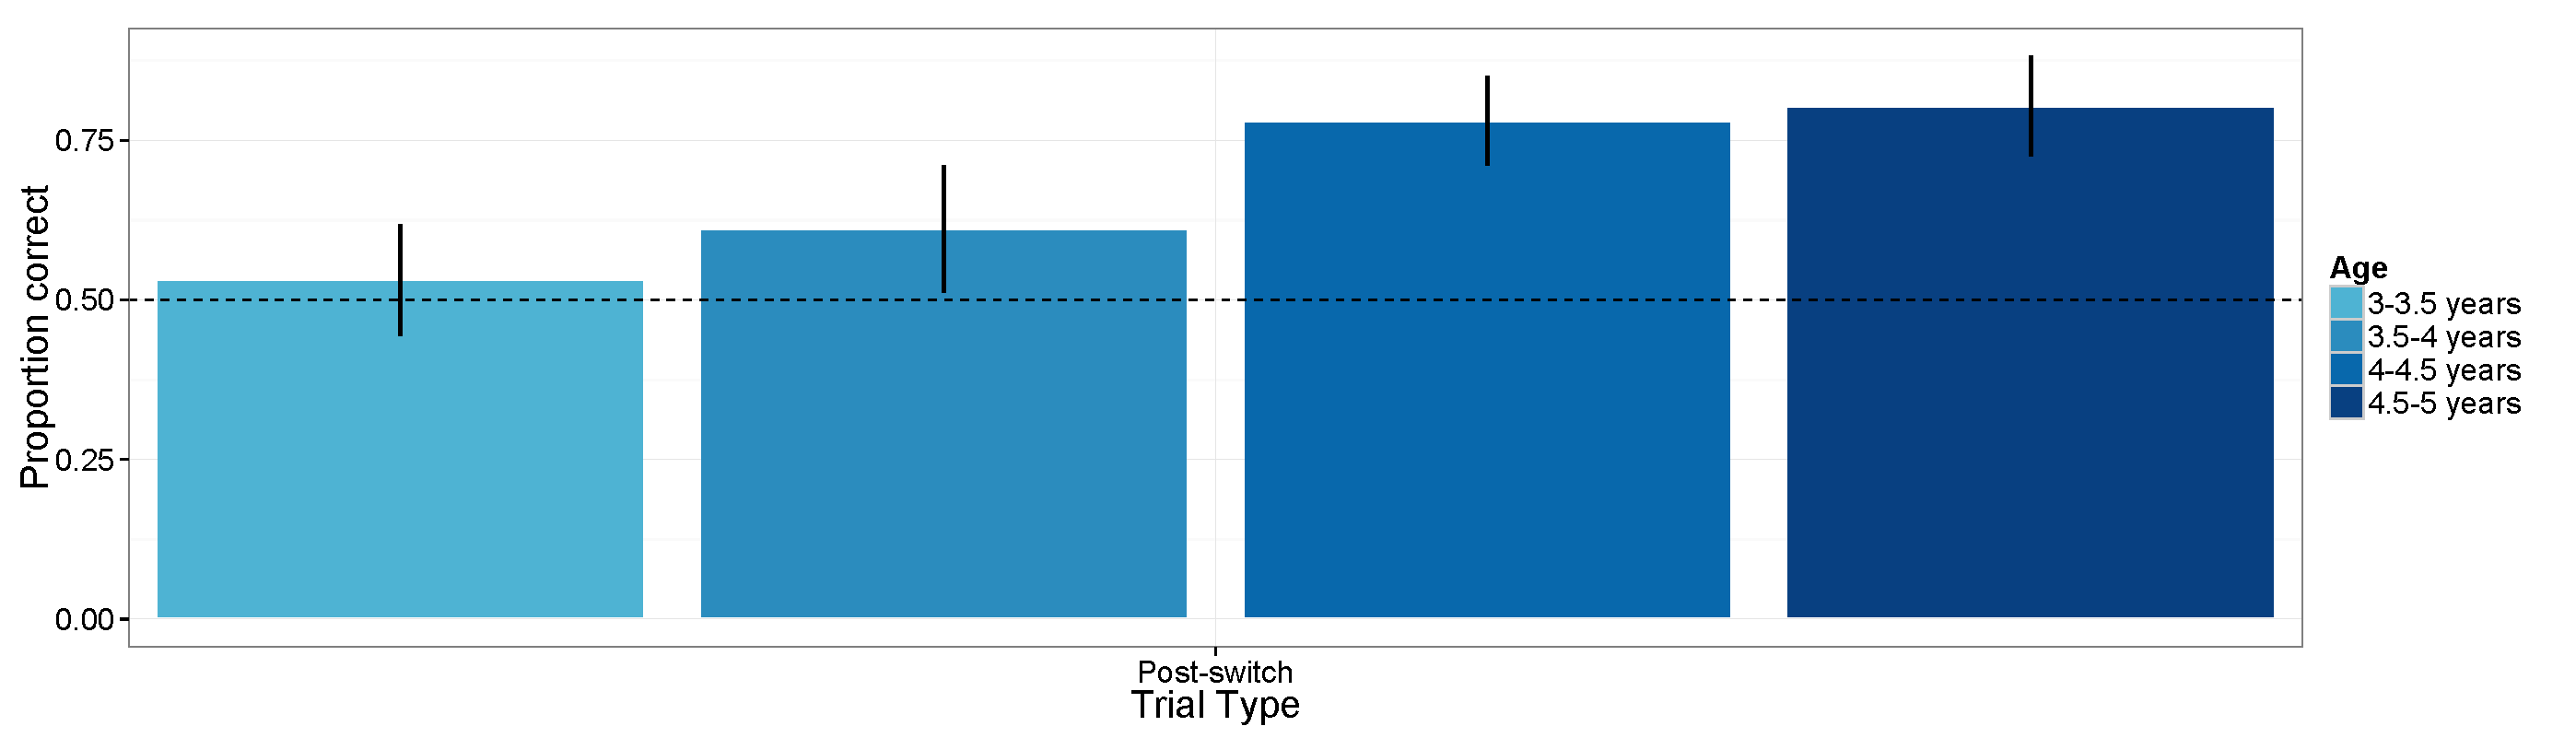
\includegraphics[scale=.5]{figures/DCCS.pdf}
%   \caption{\label{fig:exp3_DCCS} Proportion of correct responses by each age group in post-switch trials of DCCS. Error bars show 95\% confidence intervals computed by non-parametric bootstrap.}
%  \end{center}
% \end{figure}

We next turned to whether children's lower and correlated performance on ``some'' and ``none'' trials was due to an inhibitory control issue (i.e., making a response based solely on the target noun, regardless of quantifier used.)
% Accuracy on the DCCS is plotted in Figure \ref{fig:exp3_DCCS}.
Overall, we found a developmental increase in performance from three to five years of age. Performance on post-switch trials was significantly correlated with age (\textit{r} = .28, \textit{p} = .018), with 3--3.5-year-olds at chance (\emph{t}(only 4--5-year-olds performing significantly better than chance (4--4.5-year-olds: \emph{t}(18) = 3.05, \emph{p} $<$ .01; 4.5--5-year-olds: \emph{t}(16) = 3.31, \emph{p} $< $.01). After controlling for age, we did not find a significant correlation between inhibitory control and performance on either ``some'' (\textit{r} = .13, \textit{p} = .26) or ``none'' trials (\textit{r} = - .01, \textit{p} = .93) in our implicature task.

Next, we turned our attention the relation between children's performance on our scalar implicature task and quantifier knowledge. Children's performance on the Give-Quantifier task was very similar to performance on our implicature task, with all age groups performing at ceiling for the quantifier ``all'', and only older children succeeding on ``most,'' ``none,'' and ``some'' quantifier trials. Figure \ref{fig:GQ_spread} shows the breakdown of how children responded to these scalar terms. We collapsed across all age groups and found a significant bimodal distribution of responses through Hartigan's dip test in both ``some'' (\emph{D} = .19, \emph{p} $<$ .0001) and ``none'' trials (\emph{D} = .15, \emph{p} $<$ .0001). In an exploratory analysis, we ran dip tests by age group, and found that this effect was primarily driven in ``some'' trials by 3--3.5-year-olds (\emph{D} = .14, \emph{p} $<$ .0004) and 4--4.5-year-olds (\emph{D} = .13, \emph{p} $<$ .004), and in ``none'' trials by 3--3.5-year-olds (\emph{D} = .21, \emph{p} $<$ .0001) and 3.5--4-year-olds (\emph{D} = .2, \emph{p} $<$ .0001).

Overall, we found that younger children showed a bimodal and correlated pattern of response to the quantifier ``none,'' with the majority of children giving either 0 or all 8 items in these trials, and gradually shifting to a more adult-like correct response by 4.5--5 years. Similar to performance on ``some'' trials in our scalar implicature task, we found that younger children gave all 8 objects in response to the prompt ``some,'' and only the oldest age groups gave a more adult-like distribution of items in response. In a partial correlation controlling for age, we found that performance in ``none'' and ``some'' trials was significantly correlated (\textit{r} = .61, \textit{p} \textless .0001).

In partial-correlations controlling for age, we found that performance on Give-Quantifier and implicature tasks was correlated. Children who tended to struggle with scalar terms in the context of implicatures also had lower performance when asked to produce a number of items in response to a quantifier prompt, specifically on ``some''  (\textit{r} = .27, \textit{p} $<$ .02) and ``none'' trials in both tasks {\textit{r} = .52, \textit{p} \textless .0001). We did not find a significant correlation with performance on ``some'' scalar implicature and ``none'' Give-Quantifier trials (\textit{r} = .18, \textit{p} = .14), although we did find a relation between performance on ``none'' scalar implicature and ``some'' Give-Quantifier trials (\textit{r} = .35, \textit{p} = .002).

In a further exploration of the relation between quantifier knowledge and scalar implicature performance, we examined both the particular kinds of errors that children made across both tasks, and how they were related. Figure \ref{fig:exp3_wrong} shows the breakdown of children's performance in our scalar implicature task on incorrect trials. As in Experiment 2, children exhibited evidence of making selections based solely on the target noun, regardless of the quantifier used. This result closely mirrors children's performance in our Give-Quantifier task (Figure \ref{fig:GQ_spread}), in which younger children responded in a bimodal fashion for the items ``some'' and ``none.''


\subsection{Discussion}

In Experiment 3, we explored potential factors behind children's difficulty making scalar implicatures, as well as with comprehension of the quantifier ``none.'' We combined two tasks targeting specific hypothesized areas of difficulty (inhibitory control and lack of quantifier knowledge) with our implicature paradigm in a within-subjects design to explore the relation amongst these abilities. While we found that younger children did have difficulties in our inhibitory control task, we did not find a significant relation between performance in this task and inhibitory control, at least at the level that we had statistical power to detect. We did find that children's performance on the Give-Quantifier and scalar implicature tasks were related, however, and children who failed ``some'' and ``none'' trials tended to do so across both tasks. This result indicates that quantifiers may be particularly difficult for children, even when removed from this particular scalar implicature task.

While it is clear that children struggle with quantifier comprehension, the source of this developmental difficulty is less clear. Quantifiers are a difficult class of linguistic expression to acquire, due to their non-exact and varying corresponding set sizes \citeA{hurewitz2006}. Because children's definitions of these scalar terms are not solidified in the pre-school years, it is possible that that they are not able to use and contrast quantifiers on the $<${\sc none -- some -- all}$>$ scale to succeed in making scalar implicatures. That children should struggle with the semantics of quantifiers is not wholly unexpected; 5--year-old children and adults generate different interpretations of sentences containing quantified noun phrases \citeA{musolino1998}. Other work has suggested that while children can be pushed towards adult-like interpretations of such sentences, their associated pragmatic readings of quantified noun-phrases are more tenuous than adults' \citeA{musolino2006}. In addition to grappling with the semantics of quantifiers, children  must also correctly interpret the scope involved in such utterances, which is particularly difficult for children when coupled with negation \citeA{moscati2014,musolino1998,musolino2006,zhou2009}. Thus, it seems likely that the pragmatic difficulties children face in interpreting utterances with quantifiers might be compounded by an inadequate grasp of quantifier semantics.
% It is also possible that the pragmatic contexts in which these quantifiers occur are particularly difficult to process.

%%Discussion of NP-matching strategy, per R2 suggestion
It is possible, however, that the correlation we observe between children's performance on our scalar implicature task and their quantifier knowledge might not be driven by incomplete or fragile quantifier knowledge, but rather, by appealing to a similar strategy across both tasks. Recent work has shown that that 5--year-olds make scalar implicatures at adult-like levels when presented with either \emph{some} and \emph{all} or \emph{some} and \emph{none} when controlling for semantic knowledge of quantifiers \citeA{skordos2014,skordos2016}. While this result indicates that children seem to consider both ``all'' and ``none'' alternatives against which to compare the weaker quantifier ``some,'' it is unclear whether this contrast remains as salient when considering all three quantifiers together. If children are able to compute implicatures along both the \emph{some/all} and \emph{some/none} scale, but fail to do so along \emph{none/some/all}, it may point to the inclusion of both stronger alternatives decreasing the salience of the other's contrast with the weaker ``some.'' 

In such a situation, therefore, children might choose to disregard the information provided by the quantifiers as underinformative, and thus resort to ignoring the quantifiers completely in all cases, choosing to respond based solely on the noun phrase (NP) in each trial. For children whose quantifier knowledge is more fragile, relying on such a strategy might be more likely. Given the task similarities between our scalar implicature task and Give-Quantifier, it is possible that children who are recruiting this strategy for one task might also be likely to do so for the other. 

The use of this common strategy for both tasks would naturally lead to a strong correlation between scalar implicature performance and quantifier knowledge, but not between either task and the DCCS. While we believe that the DCCS requires children to employ a similar strategy in both our scalar implicature and Give-Quantifier tasks (namely, inhibiting a response by explicitly attending to the pertinent linguistic information), the two tasks differ in that children only have linguistically available to them the relevant dimension along which to sort the card. Thus, children could not apply the NP-matching strategy here. 

The question, therefore, is whether the full set of alternatives in our scalar implicature task (\emph{none/some/all}) in fact obscures the relevant contrast between the alternatives. If this is the case, then children's poor performanc in our task might not be reflective of their pragmatic abilities, but rather the result of a task-specific NP-matching strategy. To explore this possibility, we ran an additional control study on our scalar implicature task including only ``some'' and ``none'' as lexical alternatives. 

\section{Experiment 4} 

To explore whether children's lower performance on our scalar implicature task was driven by the inclusion of two relevant alternatives (``all'' and ``none''), we conducted a separate control study including only one relevant lexical alternative (``all'') to increase the salience of its contrast to the weaker ``some.'' Given our previous results showing generally poor performance on this task with younger children, and other work showing adult-like scalar implicature computation with older children \citeA{skordos2014,skordos2016}, we included only 4--5-year-olds in our sample. 

\subsection{Methods}

\subsubsection{Participants}
Table \ref{tab:exp_4_demo} shows the demographic information for a new sample of 38 participants from a local children's museum. Of the children included in the sample, the majority were identified by caregivers as White (N = 17), asian (N = 12), multiracial (N = 5) or other (N = 4). Twenty-four additional children were run but not included in analyses due to low English exposure (< 75\%), being outside of age range, or parental interference. Two children in our sample have one trial each excluded from analysis due to experimenter error. Testing took place in a small room away from the main museum floor.

\subsubsection{Stimuli}
Stimuli came from the scalar implicature task used in Experiments 1--3. The only modifications made were reducing the number of total trials to 12, with six trials per quantifier (``some'' and ``all''), which meant removing 6 total test trials from our full stimulus set. Once again, we randomly assigned participants to one of three lists, which pseudo-randomized quantifier order and controlled for position of the correct book referent. To completely control for correct referent location, we repositioned several book covers in the original stimulus set. 

\subsubsection{Procedure}
Procedure was identical to Experiments 1--3. 

\section{Results}
When presented with only ``some'' and ``all'' as alternatives in this task, 4--5-year-olds performed significantly worse on implicature trials, both in comparison to ``all'' (\emph{t}(74) = -15.972, \emph{p} < .0001), and ``some'' trials in Experiment 3 (4--4.5-year-olds: \emph{t}(34) = 2.19, \emph{p} = .035; 4.5--5-year-olds: \emph{t}(36) = 3.7, \emph{p} = .0007). Figure \ref{fig:exp4_si}) shows mean correct for each trial type and age group. An independent t-test did not reveal a significant difference for performance between age groups for either ``all'' (\emph{t}(36) = .5, \emph{p} = .62) or ``some'' (\emph{t}(36) = -0.23, \emph{p} = .82). When making an incorrect selection on ``some'' trials, children overwhelmingly chose the book consistent with ``all'' (N = 186 trials, out of a total 190 incorrect), while choosing the book consistent with ``none'' only once.  

We next fit a generalized linear mixed effects model predicting a correct response as an interaction of age and prompt. The model specifications are as follows: ({\tt{correct $\sim$ trial\char`_type * age + (trial\char`_type | subject\char`_ID)}}). Age was centered for ease of model fit. We found a significant negative effect of age, such that performance was significantly worse on ``some'' trials in comparison to ``all'' ($\beta$ = -11.19, \emph{p} < .0001). There was no significant interaction between age and trial type. 

\section{Discussion}
In Experiment 4, we tested the hypothesis that the inclusion of ``none'' in our referent-selection task decreased the saliency of the contrast between ``some'' and ``all,'' prompting children to disregard underinformative quantifier information, and resort instead to NP-matching strategy. Surprisingly, we found that excluding ``none'' as a lexical alternative in this task actually significantly reduced performance in our oldest age group. 

This finding is interesting for several reasons. First, it indicates that ``none'' is under consideration as an alternative when drawing a scalar implicature from ``some.'' When children are familiar with the semantics of ``none,'' and when it is available as an alternative, children actually benefit from its inclusion in this task. Second, these results suggest that the inclusion of another alternative might help ``unstick'' children from their bias towards choosing ``all'' in our task. Some recent work using the same task has suggested that children might have to overcome such a bias in making scalar implicatures \citeA{schneider2016}. Third, children's strikingly poor performance in our task highlights that it is more demanding than others using only ``some'' and ``all'' \citeA<cf.>{skordos2016}. 

Overall, we did not find evidence to suggest that the inclusion of ``none'' in our task hindered children's performance in making scalar implicatures. Rather, we found quite compelling evidence that its inclusion actually \emph{helps} children in our task, and may overtly draw their attention to an alternative that should be under consideration during this computation. 

\section{General Discussion}

%We designed a simple task to investigate patterns of pragmatic development both within- and between-subjects. We minimized task demands by asking participants to select the speaker's intended referent from among three visual alternatives. In Experiment 1, we replicated the finding that preschoolers can compute ad-hoc implicatures \citeA{stiller2015}, though we found poor performance on scalar implicatures. In Experiment 2, we removed competing ad-hoc descriptions from our implicature task, and found marginal increases in preschoolers' comprehension of all scalar quantifier terms. We still observed correlated difficulty with the quantifiers ``some'' and ``none,'' however. In Experiment 3, we explored two possible explanations for this pattern of performance, inhibitory control and quantifier knowledge, and found evidence that children's difficulties on our implicature task are rooted in a lack of quantifier knowledge, rather than inhibitory control. Our findings suggest that while 4-year-olds are able to compute scalar implicatures with support from contextual cues, their performance is fragile.

Why do children continue struggle to compute scalar implicatures despite their success in other pragmatic domains? Here, we designed a simple task to investigate patterns of pragmatic development involved in making scalar implicatures both within- and between-subjects. We minimized task demands by asking participants to select the speaker's intended referent from among three visual alternatives. In Experiment 1, we replicated the finding that preschoolers can compute ad-hoc implicatures \citeA{stiller2015}, though we found poor performance on scalar implicatures. In Experiment 2, we removed competing ad-hoc descriptions from our implicature task, and found marginal increases in preschoolers' comprehension of all scalar quantifier terms. We still observed correlated difficulty with the quantifiers ``some'' and ``none,'' however. In Experiment 3, we explored two possible explanations for this pattern of performance, inhibitory control and quantifier knowledge, and found a significant relation between children's knowledge of quantifiers and their performance in our implicature task, but not between inhibitory control and scalar implicature performance. In Experiment 4, we found that the inclusion of ``none'' as a lexical alternative in our task significantly improves, rather than inhibits, scalar implicature computation. Taken together, our work suggests that at least some of the difficulties children encounter when making scalar implicatures lie in their fragile grasp of the quantifiers involved. Thus while 4 and 5--year-olds are able to compute scalar implicatures with support from contextual cues, incomplete quantifier semantic knowledge may cause failures when making such pragmatic inferences.

Our work contributes to the existing literature in a number of ways. First, it offers a novel paradigm that is less complicated than many other implicature tasks, leading us to feel more confident that our results reflect children's true sensitivity rather than inadvertent task demands. Each test set remained visible to children, and they were merely asked to select which picture they thought was the referent corresponding to the speaker's description. Second, the relatively high number of trials for each participant both helped increase the precision of our measurements and also offered the possibility for children to identify lexical alternatives as the study progressed. Third, we were able not only to compare performance across age groups, but also to examine individual patterns of responses across the different trial types. This design helped us determine that preschoolers' performance on scalar implicature trials was bimodal and highly related to their performance on ``none'' trials, which we would have been unlikely to uncover in a purely between-subjects implicature design without controls. Finally, we were able to test two hypotheses about the sources of children's difficult with scalar implicatures, and found evidence for a link between poor quantifier knowledge and the ability to make scalar implicatures.

Our findings provide some support for the Alternatives Hypothesis \citeA{barner2010,barner2011}. In particular, our ad-hoc trials in Experiment 1 show that preschoolers had no difficulty generally making inferences about contextual descriptions when alternative nominal descriptions were obvious from the context. In addition, the presence of ad-hoc trials decreased scalar performance in Experiment 1 compared with Experiment 2, suggesting that children might have recognized the ad-hoc descriptions as alternatives that competed with the quantifiers.

%These results support the idea that children's ability to compute implicatures relates to their ability to reason about what other possible utterances a speaker could have used instead.

On the other hand, another pattern in our data was more difficult to reconcile with the Alternatives Hypothesis: Children's performance did not change over the course of either experiment. We had expected that, if children's difficulties with scalar implicature were due to a lack of recognition of the contrastive relation between ``some'' and ``all,'' that this relation would be revealed by the two words' consistent use in contrasting references over the course of the many trials that each child completed  \citeA<cf.>{skordos2016}. The lack of trial order effects we observed could indicate that children in our task did not yet have strong enough comprehension of these terms for contrastive use to matter, or alternatively that our referent-selection task eliminated the problem of summoning the contrasting term to mind and instead foregrounded other inferential issues.

Further, the correlated responses for ``some'' and ``none'' trials in both Experiments 1 and 2 suggested that children's difficulty with these quantifiers could have a common root, either in quantifier knowledge or inhibitory control. Our data in Experiment 3 provided evidence against a purely inhibitory account, leaving the quantifier knowledge hypothesis as one possible contender. Although ``none'' is not typically considered part of the same Horn scale as ``some'' and ``all,'' it is nonetheless a salient member of the same lexical class. Recent work has suggested that ``none'' is in fact a salient inferential alternative, at least in some models of implicature \citeA{franke2014}. Additionally, recent developmental work has indicated that, when controlling for quantifier semantic knowledge, 5--year--old children make scalar implicatures with ``some''  at adult-like levels when it is contrasted with ``none'' \citeA{skordos2014, skordos2016}. These results indicate that for children who are familiar with these quantifiers, ``none'' is a relevant alternative to ``some'' that is compared along the same lexical scale when drawing an implicature. This is further underscored by children's striking failure in Experiment 4 when ``none'' was not included as an alternative. Thus, perhaps the strong correlation we observed between ``some" and ``none'' is in fact due to the incomplete semantic knowledge for ``none'' leading to failures. In other words, if children either don't know or can't process all the quantifiers in the lexical class, they may fail to reason appropriately about implicatures.

%Our results suggest that children's difficulties computing scalar implicatures lie in incomplete quantifier knowledge, and that children who failed to make implicatures similarly struggled in comprehending the quantifier scale. While our findings are generally consistent with the Alternatives Hypothesis, we suggest that quantifier knowledge is a bottleneck which constrains children's ability to recognize and contrast relevant lexical alternatives in generating implicatures.

%NOTE: THIS NEEDS MORE WORK - WANT TO DISCUSS CONNECTIONS TO PREVIOUS QUANTIFIER RESULTS HERE
Here, we found that children's ability to compute scalar implicatures correlated with their quantifier knowledge, but not with inhibitory control. While our findings are generally consistent with the Alternatives Hypothesis, we suggest that quantifier knowledge is a bottleneck which constrains children's ability to recognize and contrast relevant alternatives along a lexical scale when making scalar implicatures. Based on the results from this work, incomplete quantifier knowledge, rather than pure inhibitory control, is at least one factor driving children's struggles with scalar implicatures. Quantifiers as a lexical class are surprisingly difficult to acquire \citeA<cf>{hurewitz2006}, and it is unsurprising that preschoolers grapple with their meanings until fairly late in development. 

It is highly probable, however, that children's pragmatic difficulties in this domain do not lie solely in quantifier semantics, but may be influenced by other factors, and further empirical work is needed to pursue these directions. While we do not find evidence of a link between scalar implicatures and inhibitory control in this or other work \citeA{nordmeyer2016}, there are many different components of executive function; it is possible that an as-yet untested feature of this construct might play a more significant role in children's performance. For example, we did not record children's response time on the scalar implicature task. Perhaps a response latency measure might yield more information about the particular processing and inhibitory demands of scalar implicatures. 

%NOTE: THIS NEEDS TO BE EDITED AFTER CONTROL STUDY
Additionally, our quantifier knowledge measure \citeA{barner2009} may present many of the same pragmatic hurdles as our implicature task. The syntactic construction of prompts in Give-Quantifier are very similar (e.g., ``Can you put \emph{some} of the oranges on the plate?'' vs. ``On the cover of my book, \emph{some} of the pictures are oranges.''). This similarity may also prompt children with low quantifier knowledge to rely on a similar NP-matching strategy in both tasks, leading to the observed relationship. Although we tried to control for this in Experiment 4, we did not explicitly test relation between children's performance on the Give-Quantifier task there, and more work is needed to pursue this possibility.

Another possible explanation for children's lower performance on ``some'' and ``none'' in both our scalar implicature and Give-Quantifier tasks may be the slightly lower age in our sample compared to other studies using a similar design \citeA{skordos2014,skordos2016}. While we do find that the oldest children in each of our samples perform significantly worse with these two quantifiers in comparison to ``all'' across Experiments 1--3, we are testing slightly younger children ($<$ 5 years) in comparison to \citeA{skordos2016} (5--5.5 years). While in a tablet adaptation of this paradigm which included 24 5--6.5-year-olds we again found significantly lower performance with these two quantifiers, we also found significantly lower performance on scalar implicatures overall, perhaps due to the non-social nature of the tablet design \citeA{schneider2016}. Further, in Experiment 4, we found significantly lower performance in 4--5-year-olds in comparison to Experiments 1-3, indicating that this task is likely more difficult for participants. Although we controlled for age here in our analyses, future work should expand the sample age range to rule out general trends of pragmatic development.

%NOTE - ADD MORE DETAILS ABOUT THE EFFECTS OF MULTIPLE SCALES
It is also possible that, similarly to adults, children's scalar implicature performance may also be affected by non-scalar alternatives, such as ``one'' or ``two'' \citeA{degen2015}. Indeed, children show some evidence of comprehending quantifiers like ``some'' and ``none'' when presented in the same truth-value judgment task as exact number terms \citeA{barner2009}. Future work should explore other more distinct measures of quantifier semantics, as well as the role of other alternatives involved in making scalar implicatures.

%In sum, our work suggests that children can draw implicatures based on some lexical choices---such as in the case of ad-hoc implicatures---but they still struggle with quantifier-based scalar implicatures until relatively late. This trouble with quantifiers is not confined to making scalar implicatures, but extends to children's knowledge of the quantifier ``none'' as well.

In sum, our work suggests that children can draw implicatures based on some lexical choices---such as in the case of ad-hoc implicatures---but they still struggle with quantifier-based scalar implicatures until relatively late. The results reported here do not rule out alternative or additional factors at work in children's struggles with scalar implicatures, however, and future work should investigate these possibilities. We do find strong evidence here, however, that lack of quantifier knowledge is at least partially responsible for children's extended difficulties with scalar implicatures.

\section{Tables and Figures}

\newgeometry{margin=1cm}
\begin{landscape}
\begin{table}[!ht]
\footnotesize
\centering
\begin{tabular}{| p{2.2cm} | p{2cm} | p{1.69cm} | p{4.5cm} | p{5cm} | p{7.2cm} |} \hline
{\bf Study} & {\bf Scale(s)} & {\bf Ages} & {\bf Measure} & {\bf Sentence Type} & {\bf Main Finding} \\ \hline
Noveck (2001) & non-necessity--necessity, possibility--impossibility, some--all & 5;1--5;11, 7;1--8;0, 9;0--9;5, 10;0--11;7 & Truth Value Judgment (\textit{Yes, I agree} or \textit{No, I do not agree}) & ``Some giraffes have long necks'' & \parbox[t]{7.2cm}{Comprehension matters: Children demonstrate\\ pragmatic competence by age 7 in evaluating a variety of plausible and implausible sentences.} \\ \hline
\parbox[t]{2.2cm}{Papafragou \&\\Mussolini (2003)} & \parbox[t]{2cm}{some--all,\\two--three,\\start--finish} & \parbox[t]{1.69cm}{4;11--5;11\\(Study 1)\\5;1--6;5\\(Study 2) } &  \parbox[t]{4.5cm}{Felicity Judgment (\textit{Did Minnie\\answer well?})} & ``Some of the horses jumped over the fence'' (when all of the horses jumped over the fence) & Support matters: Children were more likely to reject infelicitous weak descriptions for numbers, and for all types of weak descriptions in the task with more pragmatic support (informativeness training, context of competition, statements about specific events). \\ \hline
\parbox[t]{2.2cm}{Papafragou \&\\Tantalou (2004)} & some--all, ad-hoc, encyclopedic & 4;1--6;1 & Felicity Judgment (Decide whether or not to award a speaker a prize) & \textit{Did you color the stars?} ``I colored some" (when all were colored) & Scales matter: Children mainly withheld prizes for weak descriptions, and at higher rates for ad-hoc trials than other trial types. \\ \hline
\parbox[t]{2.2cm}{Guasti, Chierchia, Crain, Foppolo, Gualmini,\\\& Meroni (2005)} & some--all & 7;0--7;7 & Truth Value Judgment: \textit{Yes, I agree} or \textit{No, I do not agree} (Studies 1--3), \textit{Did Carolina say the wrong thing?} (Study 4) & ``Some giraffes have long necks'' (replication of Noveck (2001)), and scene descriptions, e.g. ``Some monkeys are eating a biscuit'' (when all are) & Context matters: 7-year-olds reliably compute implicatures for ``some'' after a training that increased their sensitivity to the informativeness of speakers' descriptions (e.g., calling a grape ``fruit'' instead of ``grape'') and when contextualized as evaluating a novice speaker describing a scene.\\ \hline
Miller, Schmitt, Chang, \& Munn (2005) & some--all & \parbox[t]{1.69cm}{4;1--5;5\\(Study 1)\\ 3;6--5;10\\(Study 2)} & \parbox[t]{4.5cm}{Direct Instruction Task\\(Study 1);\\Picture Matching Task\\(Study 2)} & ``Make some faces HAPPY/Make SOME faces happy/Make some HAPPY faces'' (Study 1), ``Show me where Pete made some faces HAPPY/Show me where Pete made SOME faces happy'' & Prosody matters: In both tasks (completing the scene or selecting the referent), children reliably identified only a subset of the faces (out of four) when ``some'' was stressed, but not when it was unstressed.\\ \hline
\parbox[t]{2.2cm}{Huang \&\\Snedeker (2009)} & \parbox[t]{2cm}{some--all,\\two--three} &\parbox[t]{1.69cm}{5;2--6;1\\(Study 1)\\5;5--6;9 \\(Studies 2\\\& 3)} & \parbox[t]{4.5cm}{Eye-tracking\\referent selection} & ``Point to the girl with some of the socks'' (when other girls and boys have shares of socks and soccer balls) & Time scale matters: Across studies, children were delayed in identifying the referent for scalar implicature trials, and accept and overlap between the meaning of ``some'' and ``all.'' \\ \hline
Katsos \& Bishop (2011) & some--all, ad-hoc & 5;1--6;3  & \parbox[t]{4.5cm}{Binary Truth Value Judgment\\(Study 1); Ternary Truth\\Value Judgment (Study 2);\\Sentence-to-picture Matching Task\\(Study 3)} & ``The mouse picked up some of the carrots'' & Measures matter: While children tended to a accept under-informative scalar and ad-hoc descriptions given a binary decision, they showed sensitivity to weaker statements given a ternary choice or picture matching task. \\ \hline
Barner, Brooks, \& Bale (2011) & some--all, ad-hoc & 4;0--5;0 &Truth Value Judgment & ``Are some of the animals sleeping?'' (when all are) & Specificity matters: 4-year-olds accept weak ad-hoc and scalar descriptions. When preceded by restrictive ``only'', they reject ad-hoc descriptions but continue to accept that ``only some'' can mean \emph{all}.\\ \hline
\parbox[t]{2.2cm}{Skordos \&\\Papafragou (2014)} & some--all & 4;9--5;8 & Felicity Judgment (\textit{Did the puppet answer well?}) & ``Some of the blickets have a crayon'' (when all of them do)  & Comparisons matter: Children were more likely to reject infelicitous uses of ``so'' if they first heard ``all'' falsely refer to quantity (only 3/4 blickets had crayons), but not if ``all'' referred falsely to the objects (e.g., ``all of the blickets have a scarf'').\\ \hline \end{tabular}
\caption{\label{tab:lit_review}Review of previous literature on children's comprehension of implicatures.}
\end{table}
\end{landscape}
\restoregeometry

\begin{table}[tb]
\centering
\begin{tabular}{ccccccc}
\hline
{\bf Age group} & {\bf N} & {\bf N Female} & {\bf N Male} & {\bf Mean} & {\bf Median} & {\bf SD} \\
\hline
4.0 -- 4.5-year-olds & 24 & 12 & 12 & 4.2 & 4.19 & 0.14 \\
4.5 -- 5.0-year-olds & 24 & 17 & 7 & 4.74 & 4.73 & 0.16\\
\hline
\end{tabular}
\caption{\label{tab:exp_1_demo}Participant age information for Experiment 1.}
\end{table}

\begin{figure}
 \begin{center}
  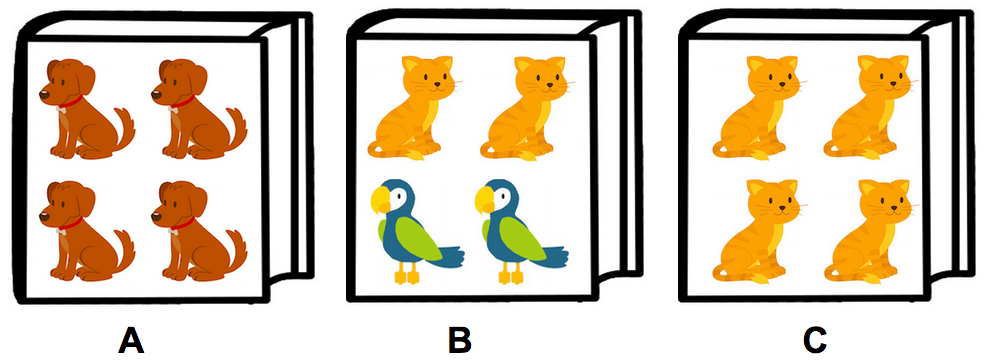
\includegraphics[height=2in]{figures/implicatures_demo_letters.png}
  \caption{\label{fig:demo} Example trial stimuli used in all experiments. Children received a clue from the experimenter about which book she had in mind and responded based solely on the clue; this was either an ad-hoc or a scalar description of a book with either an unambiguous or implicature target.}
 \end{center}
\end{figure}

 \begin{table*}
 \footnotesize
 \centering
     \begin{tabular}{C{1.5cm} C{2cm} C{1.5cm} C{1.5cm} C{4.5cm} C{1.5cm}}
                      \hline
       \null   Condition  & Trial type & \# trials, Expt. 1 & \# trials, Expts. 2 \& 3 & Statement: ``On the cover of my book, ...'' & Target   \\
       \hline
            Scalar & implicature & 4 & 6 &  ``...some of the pictures are cats'' & B	 \\
          & all  & 2 &  6 & ``...all of the pictures are cats'' & C		                 \\
           & none  & 2 & 6 & ``...none of the pictures are cats'' & A			\\
               & unambiguous `some' 	&  2 &  & ``...some of the pictures are birds'' & B					        \\
	\hline
	    Adhoc       & implicature & 4 &  & ``...there are cats'' & C 		\\
	     & distractor & 2 &  & ``...there are dogs'' & A	     \\
          & comparison & 2 &  & ``...there are birds'' & B 	   \\
       \hline
     \end{tabular}
     \caption{Study designs for Experiments 1, 2, and 3, using script examples for the stimulus set pictured in Figure \ref{fig:demo}. \label{tab:scripts} }
 \end{table*}
 
 \begin{figure}
 \begin{center}
  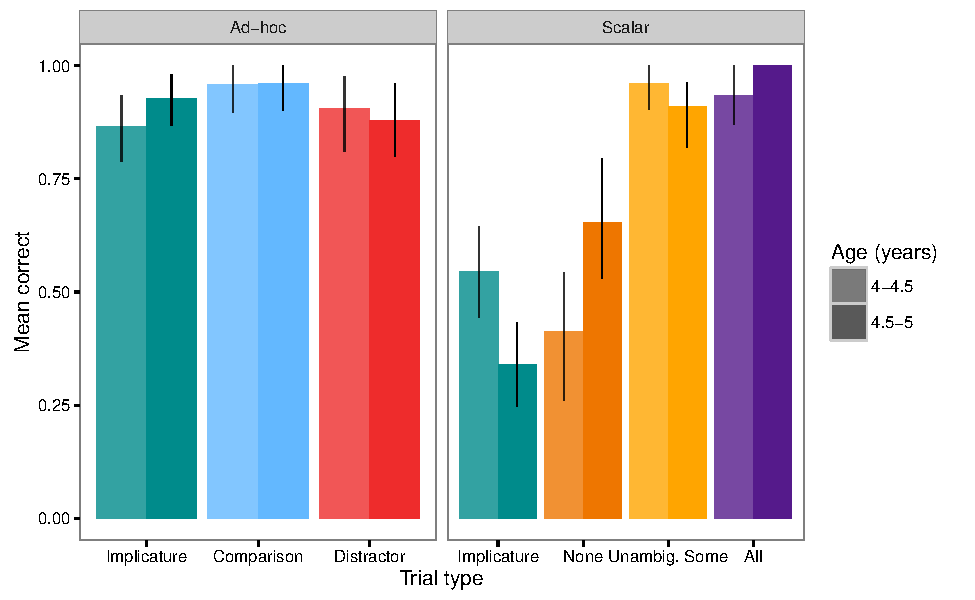
\includegraphics[width=6in]{figures/exp1_performance.pdf}
  \caption{\label{fig:exp1_perf} Proportion of correct responses by each age group across all trial types and split by implicature type. Error bars show 95\% confidence intervals computed by non-parametric bootstrap.}
 \end{center}
\end{figure}

\begin{figure}
 \begin{center}
  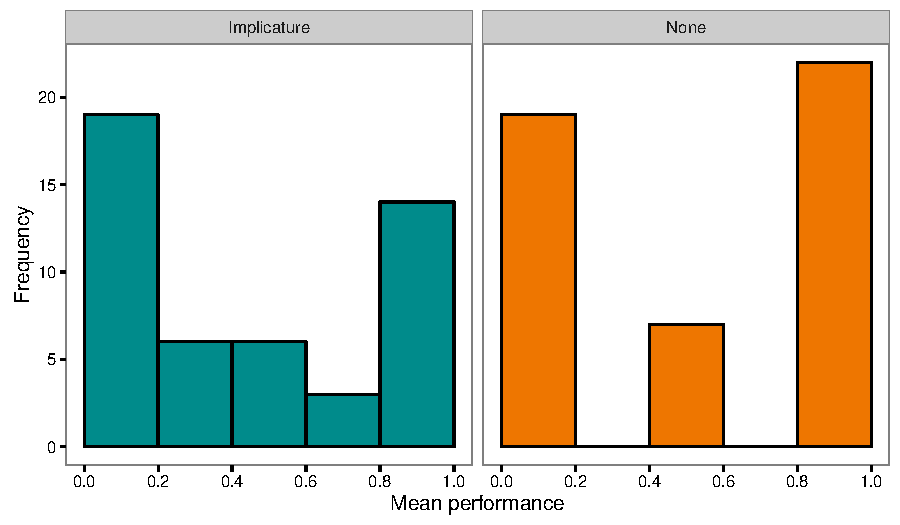
\includegraphics[width=6in]{figures/exp1_hist.pdf}
  \caption{\label{fig:imp_hist} Frequency of mean performance, split by condition.}
 \end{center}
\end{figure}

\begin{table}[tb]
\centering
\begin{tabular}{ccccccc}
\hline
{\bf Age group} & {\bf N} & {\bf N Female} & {\bf N Male} & {\bf Mean} & {\bf Median} & {\bf SD} \\
\hline
3.0 -- 3.5-year-olds & 12 & 6 & 6 & 3.4 & 3.35 & 0.1\\
3.5 -- 4.0-year-olds & 13 & 6 & 7 & 3.8 & 3.67 & 0.12\\
4.0 -- 4.5-year-olds & 14 & 9 & 5 & 4.3 & 4.24 & 0.1\\
4.5 -- 5.0-year-olds & 12 & 3 & 9 & 4.8 & 4.63 & 0.15\\
\hline
\end{tabular}
\caption{\label{tab:exp_2_demo}Participant age information for Experiment 2.}
\end{table}

\begin{figure}
 \begin{center}
  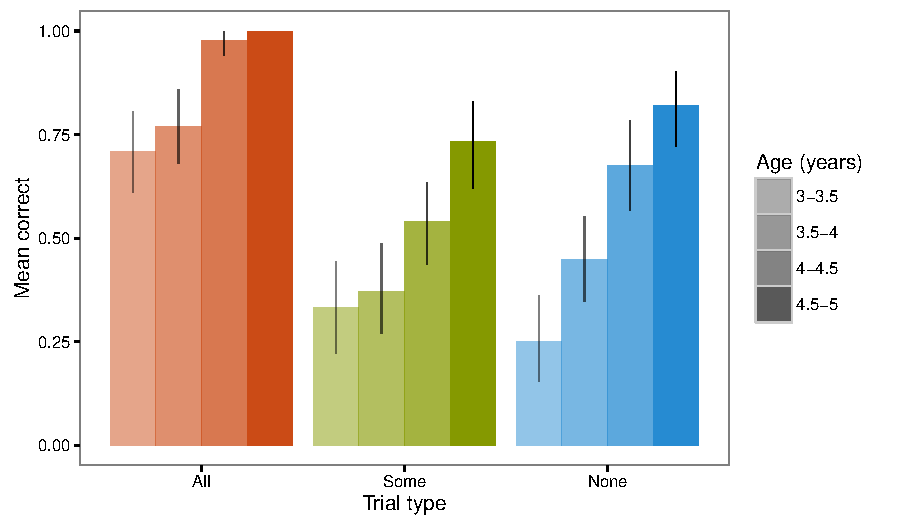
\includegraphics[width=6in]{figures/exp2_performance.pdf}
  \caption{\label{fig:exp2_perf} Proportion of correct responses by each age group across all scalar trial types. Error bars show 95\% confidence intervals computed by non-parametric bootstrap.}
 \end{center}
\end{figure}

\begin{figure}
 \begin{center}
  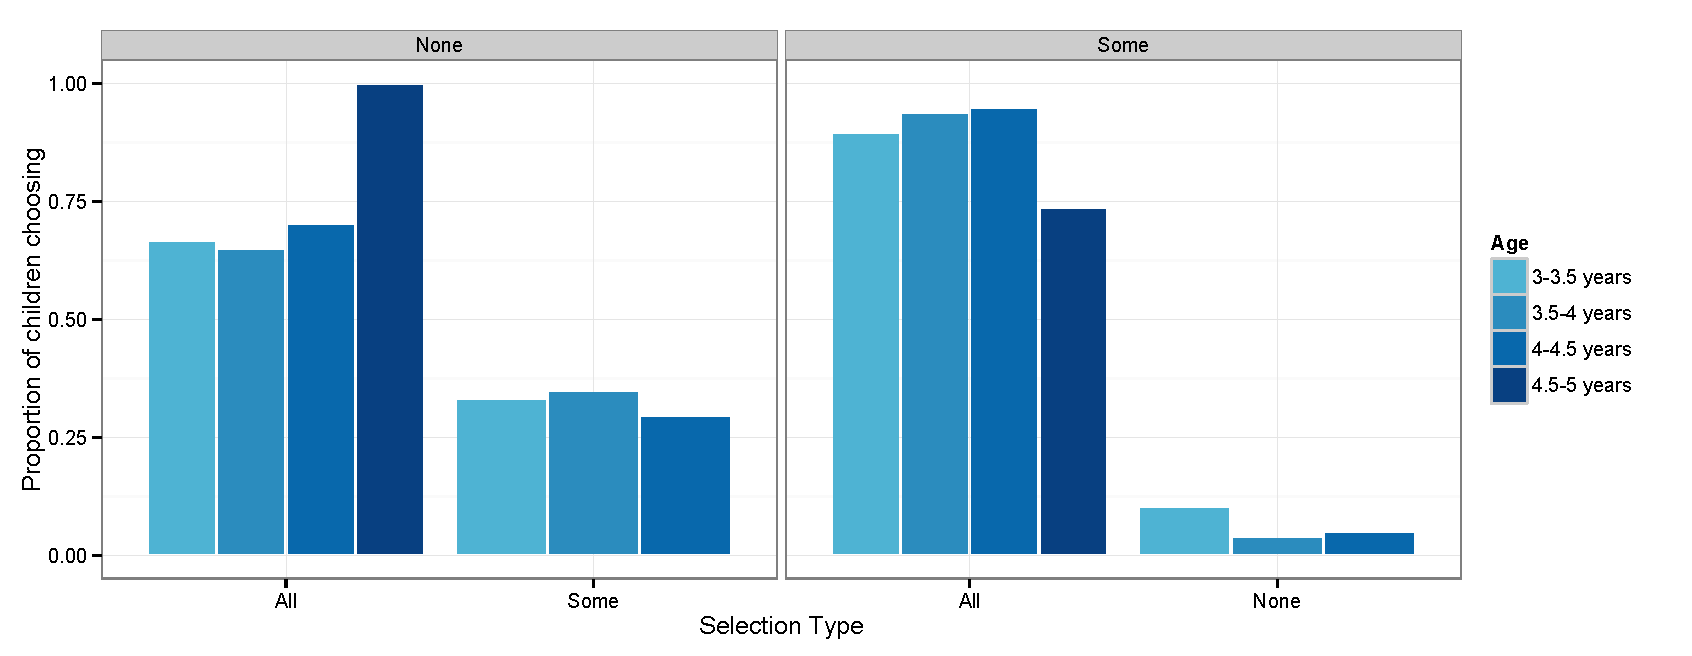
\includegraphics[width=6in]{figures/exp2_wrong.pdf}
  \caption{\label{fig:exp2_wrong} Scalar implicature error analysis. Count of children choosing an alternative on incorrect trials, faceted by trial type (``all,'' ``some,'' and ``none'') and split by age group.}
 \end{center}
\end{figure}

\begin{table}[tb]
\centering
\begin{tabular}{ccccccc}
\hline
{\bf Age group} & {\bf N} & {\bf N Female} & {\bf N Male} & {\bf Mean} &  {\bf Median} & {\bf SD} \\
\hline
3.0 -- 3.5-year-olds & 18 & 12 & 6 & 3.23 & 3.24 & 0.13\\
3.5 -- 4.0-year-olds & 18 & 10 & 8 & 3.73 & 3.8 & 0.18\\
4.0 -- 4.5-year-olds & 18 & 7 & 11 & 4.16 & 4.11 & 0.11\\
4.5 -- 5.0-year-olds & 18 & 9 & 9 & 4.7 & 4.68 & 0.14\\
\hline
\end{tabular}
\caption{\label{tab:exp_3_demo}Participant age information for Experiment 3.}
\end{table}

\begin{figure}
 \begin{center}
  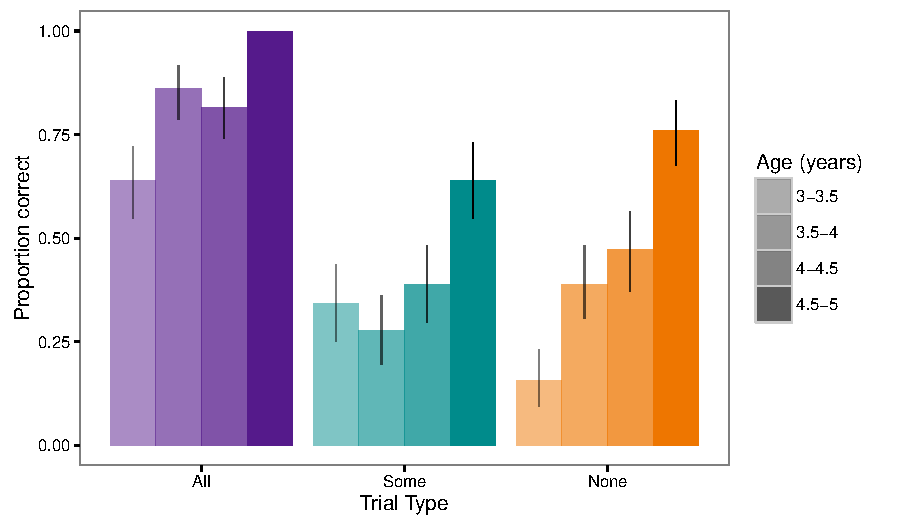
\includegraphics[width=6in]{figures/exp3_SIperformance.pdf}
  \caption{\label{fig:exp3_perf} Proportion of correct responses by each age group across all trial types for the scalar implicature task. Error bars show 95\% confidence intervals computed by non-parametric bootstrap.}
 \end{center}
\end{figure}

\begin{figure}
 \begin{center}
  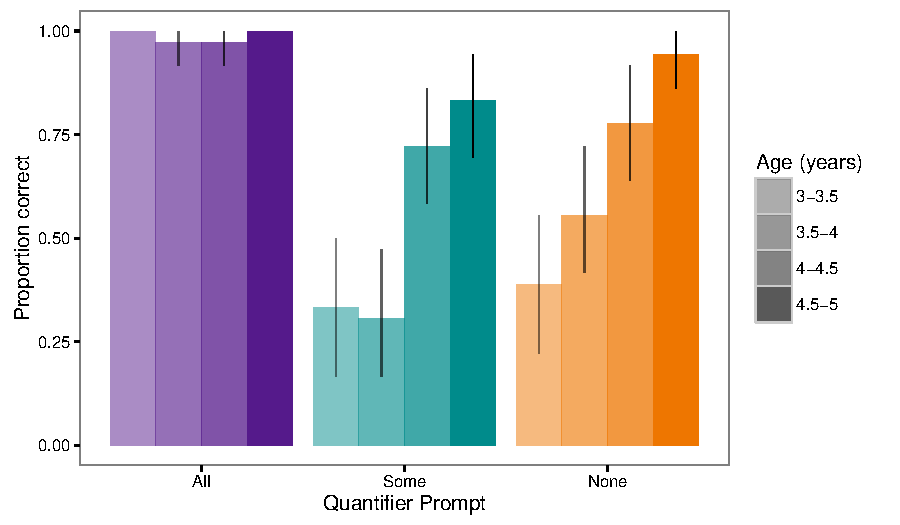
\includegraphics[width=6in]{figures/exp3_GQperf.pdf}
  \caption{\label{fig:exp3_GQright} Proportion of correct responses by each age group for the Give Quantifier task, with quantifier prompts \textit{all, most, none} and \textit{some}. Error bars show 95\% confidence intervals computed by non-parametric bootstrap.}
 \end{center}
\end{figure}


\begin{figure}
 \begin{center}
  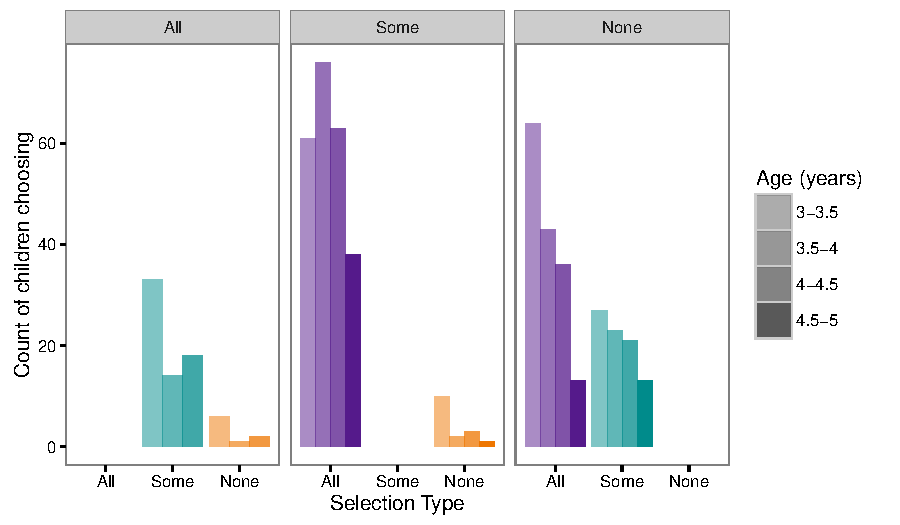
\includegraphics[width=6in]{figures/exp3_SIwrong.pdf}
  \caption{\label{fig:exp3_wrong} Scalar implicature error analysis. Count of children choosing an alternative on incorrect trials, faceted by trial type (``all,'' ``some,'' and ``none'') and split by age group.}
 \end{center}
\end{figure}

\begin{figure}
 \begin{center}
  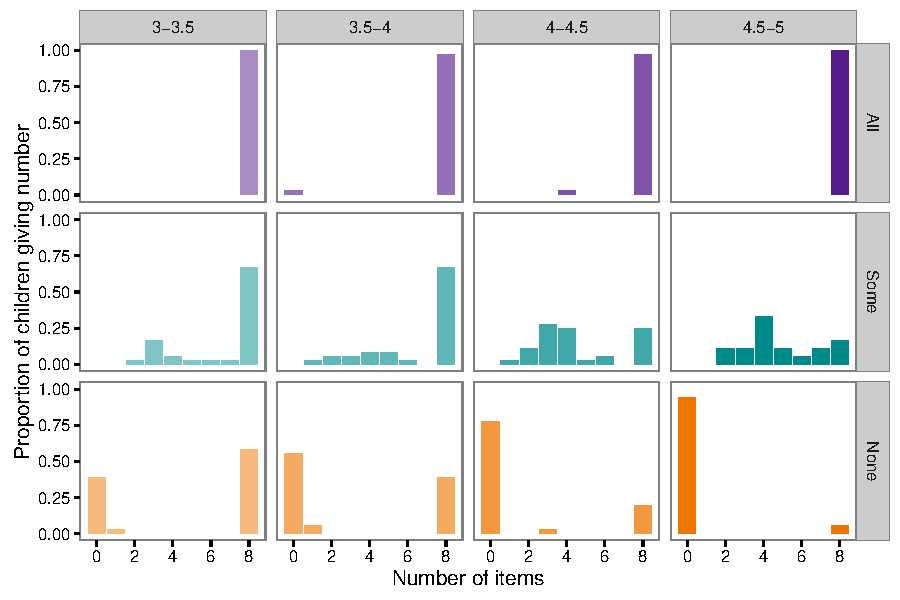
\includegraphics[width=6in]{figures/exp3_GQhist.pdf}
  \caption{\label{fig:GQ_spread} Give-Quantifier performance. Proportion of children giving numbers of items faceted by age group and quantifier prompts (``all,'' ``none,'' and ``some'').}
 \end{center}
\end{figure}

\begin{table}[tb]
\centering
\begin{tabular}{ccccccc}
\hline
{\bf Age group} & {\bf N} & {\bf N Female} & {\bf N Male} & {\bf Mean} & {\bf Median} & {\bf SD} \\
\hline
4.0 -- 4.5-year-olds & 18 & 14 & 4 & 4.22 & 4.21 & 0.14\\
4.5 -- 5.0-year-olds & 20 & 14 & 6 & 4.79 & 4.82 & 0.17\\
\hline
\end{tabular}
\caption{\label{tab:exp_4_demo}Participant age information for Experiment 4.}
\end{table}

\begin{figure}
 \begin{center}
  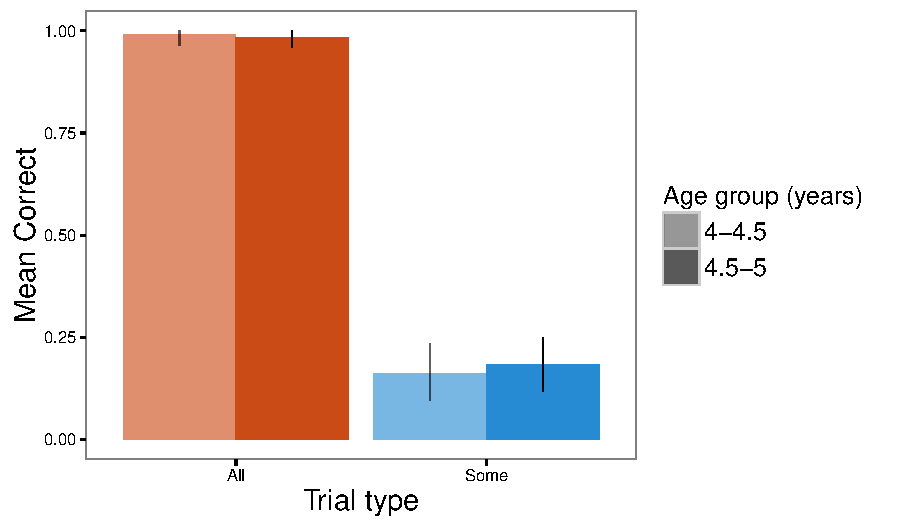
\includegraphics[width=6in]{figures/exp4_SIperf.pdf}
  \caption{\label{fig:exp4_si} Scalar implicature performance. Proportion of children giving numbers of items faceted by age group and trial type (``all,'' ``none,'' and ``some'').}
 \end{center}
\end{figure}


%
%\bibliographystyle{apacite2}
\bibliography{si_quant}

\end{document}
